\icode{E-MD-SI-L3-261115-001}
如图，吊篮 $A$、物体 $B$、物体 $C$ 的质量相等，弹簧质量不计，$B$ 和 $C$ 分别固定在弹簧两端，放在吊篮的水平底板上静止不动，将悬挂吊篮的轻绳剪断的瞬间，下列结论正确的是\paren[]

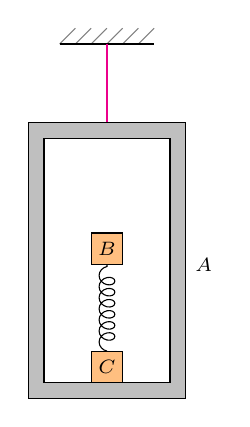
\begin{tikzpicture}[font=\scriptsize]
	\foreach \x in {-.6,-.4,...,.6}
	\draw[gray] (\x,0)--++(.2,.2);
	\draw[thick] (-.6,0)--(.6,0);
	\draw[magenta] (0,0)--(0,-1);
	\draw[fill=gray!50] (-1,-1) rectangle(1,-4.5);
	\draw[fill=white] (-.8,-1.2) rectangle(.8,-4.3);
	\draw[fill=orange!50] (-.2,-4.3) rectangle(.2,-3.9)node[midway]{\(C\)} (-.2,-2.4) rectangle(.2,-2.8)node[midway]{\(B\)};
	\draw[decoration={aspect=.8,segment length=4,amplitude=1mm,coil},decorate] (0,-3.9)--(0,-2.8);
	\node at(1,-2.8)[right]{\(A\)};
\end{tikzpicture}
\begin{choices}
	\item 吊篮 $A$ 的加速度大小为 $g$
	\item 物体 $B$ 的加速度大小为 $g$
	\item 物体 $C$ 的加速度大小为 $\frac{3}{2}g$
	\item \(A\)、\(B\)、\(C\)的加速度大小都等于\(g\)
\end{choices}
\begin{answer}
    C\qquad 提示：
\end{answer}